\chapter{Credit Mining System Design}
\label{chp:design}

% section overview, main components. Libtorrent as dependency. 
The goal of this thesis is to implement a system where it can be used to both gain credit and improve swarm performance. In this thesis, we introduce ``Credit mining system'', an automatic investment framework on swarm with multidimensional properties. With credit mining system, locally, a user can gain credit with limited bandwidth allocation without any intervention needed. We assume the \textit{credit} is the amount of bytes from the system to the community and vice versa. From higher perspective, credit mining system will help a swarm to keep alive by providing integral pieces to the peer who might need it. Although credit mining system will be implemented in Tribler system, it is possible to apply this feature to any file-sharing \bt~client.

Firstly, the dependencies of credit mining system which is \textit{libtorrent}'s s\textit{hare mode} will be elaborated. \texttt{Share mode} is a module which can be activated as an intent to helping a swarm instead of normal content downloading. This module will be explained in detail in section \ref{section:sharemode}. Afterwards, the design of credit mining system is presented. This system consists of several subroutines which will be explained in section \ref{section:cmcomponents}. 

\section{Libtorrent's share mode}
\label{section:libtorrent}
\label{section:sharemode}
\bt~is just a collection of specification. It is free to be implemented with any languages. One of most popular implementation is \textit{libtorrent}. \textit{Libtorrent} is written in \texttt{C++} and  has \texttt{python} binding. \textit{Libtorrent} started in 2003 by Arvid Norberg and it implemented most of the \bt~specification. Most of the well known extension such as DHT, PEX, magnet link, multi-tracker, and webseed also have been implemented. \textit{Libtorrent} is widely used by many torrent client such as Deluge, qBittorrent, Free download managers, and many others.

One of the crucial feature used in this work is \textit{share mode} \footnote{Core code of share mode can be found in \url{https://github.com/arvidn/libtorrent/blob/master/src/torrent.cpp\#L9586-L9727}}. Initial work performed by \citeauthor{2015:creditmining:capota} also used this feature\cite{2015:creditmining:capota}. By enabling share mode, it means that one is not interested in downloading the file in a swarm, but in gaining higher share ratio. It is done by download as little as possible and upload as much as possible. A swarm downloaded in share mode may never finish as \textit{libtorrent} only download piece of a torrent which satisfied the share mode requirements.

Share mode algorithm works heuristically as it estimates the rarest piece available in the swarm based on participated peers. The algorithm is presented in Algorithm \ref{alg:ltsharemode}. For clarity, we divide this algorithm in two part. First part is to pass all the restrictions. It tries to find missing pieces for each peers (line \ref{alg:l_lts:missingp}), disconnects some of the seeder because of connection limit (line \ref{alg:l_lts:disconnectpeers}), and reduces the number of missing pieces with twice the number of seeder (line \ref{alg:l_lts:reducemissing}). For the last, it is based on assumption that seeder can upload as fast as the system. Share mode will fail if all missing pieces are expected to be provided by the seeders (line \ref{alg:l_lts:retmis}), upload ratio could not reached (line \ref{alg:l_lts:retdlenough}), or too many parallel download (line \ref{alg:l_lts:retdling}).

Second part of share mode is to determine the rarest piece. \textit{Libtorrent} counts the number of peer for each piece to find the lowest one. The number of peer on the rarest piece is termed \textit{rarity}. Share mode ensure that it only downloads the rarest piece available (line \ref{alg:l_lts:rarepc}). We end the routine prematurely if there are not enough peer to upload the rarest piece (line \ref{alg:l_lts:rareunable}). Otherwise, it will randomly download the rarest pieces if there are more than one option (line \ref{alg:l_lts:dlrare}). 

\begin{algorithm}[h!]
	\caption{Libtorrent share mode algorithm}
	\label{alg:ltsharemode}
	\begin{algorithmic}[1]
		\Require{$T$ as share mode target}
		\Statex \hrulefill \Comment{Part 1}
		\State{$missing\_piece \gets 0$}
		\ForAll{$p \in connected\_peers$}
		\If{$p$ is a $leecher$ $and$ $p$ is not in share\_mode}	
		\State{$missing\_pieces$} += {$total\_pieces - pieces(p)$} \label{alg:l_lts:missingp}
		\EndIf	
		\EndFor
		\If{$|connected\_seeders|$ in $connected\_peer$ $>$ $90\%$}	
		\State disconnect excess seeder \label{alg:l_lts:disconnectpeers}
		\EndIf
		\State{$missing\_pieces$} -= {$2 \times |connected\_seeders|$}	\label{alg:l_lts:reducemissing}	
		\If{$missing\_pieces \leq 0$}  \label{alg:l_lts:retmis}
		\State \Return 
		\EndIf
		\If{$num\_downloaded \times T > uploaded$} \label{alg:l_lts:retdlenough}
		\State \Return
		\EndIf
		\If{$downloading > 5\% \times num\_downloaded$} \label{alg:l_lts:retdling}
		\State \Return
		\EndIf
		\Statex \hrulefill \Comment{Part 2}
		\State{$rarest\_rarity \gets MAX\_INTEGER$} 
		\ForAll{$pc \in pieces()$}
		\If{$pc$ not in $collected\_piece$ $and$ $peer\_count(pc) \leq rarest\_rarity$ }	\label{alg:l_lts:rarepc}
		\State{$rarest\_rarity \gets peer\_count(pc)$} 
		\State{$rare\_piece$.push($pc$)}
		\EndIf	
		\EndFor
		\If{$|connected\_peers| - rarest\_rarity < T$} \label{alg:l_lts:rareunable}
		\State \Return
		\EndIf
		\State download {$random(rare\_piece)$} \label{alg:l_lts:dlrare}
	\end{algorithmic}
\end{algorithm}

There are two limitations on this feature as we observed. Firstly, share mode did not check whether a swarm is good enough to perform this operation. It only tries to find popular pieces regardless of the swarm condition. It has high possibilities that swarm with poor capacity will have very low uploading rate. The bandwidth used to check torrent pieces is wasted and the ``investment'' will not go well. Therefore, user is responsible of whether share mode will yield high credit or not.

Secondly, the biggest limitation of share mode is the possibilities of getting bottleneck because of its strict policy. In early stage of joining a swarm, share mode downloaded very few pieces at a time. For example, until the system has downloaded at least 20 pieces, it will only download 1 piece (5\%) at a time in share mode (line \ref{alg:l_lts:retdling}). It is also necessary to wait that single piece to be uploaded (line \ref{alg:l_lts:retdlenough}) to at least $T$ peers. The combination of line \ref{alg:l_lts:retdlenough} and \ref{alg:l_lts:retdling} can result in slower decision making and the rarity of pieces may have changed. If the system is too late to completely receive piece, or the piece is not uploaded fast enough, this piece could be obsolete as nobody wants it anymore. Therefore, the condition in line \ref{alg:l_lts:retdlenough} may never be satisfied. If other pieces could not cover this condition (by uploading to more than $T$ peers), then share mode unable to continue. The system then will not download nor upload any pieces anymore.

\section{Credit Mining Architecture}
\label{section:cmcomponents}

Credit mining system is intended to do its task automatically with minimal user intervention. The way this system designed is to align supply and demand of chosen swarm. Short term advantage of this approach is to gain credit by minimizing download and maximizing upload. In the long term, this potentially increase overall performance of other user as well.

The system can be implemented on any torrent client. In Figure \ref{fig:cmcomponents}, it shown the compulsory elements and the relation between \textit{credit mining system} and \textit{torrent client}. Currently, we assume that every torrent client also track how much data a user has been downloaded and uploaded in \textit{credit storage}. Naturally, any torrent client must have \textit{Torrent client downloader} module as well. \textit{Libtorrent} library also must exist as part of dependencies. Other required feature is the ability of discovering peer by all method (DHT, PEX, LSD, etc). In some cases, peer discovery function is disabled for security reasons. While disabling one should not affect credit mining system, it will reduce overall prospecting accuracy.

Credit mining system consists of several elements. Those are \textit{credit mining manager}, \textit{miners}, \textit{mining sources}, \textit{settings} object, and \textit{predownloader}. The \textit{manager} receives the \textit{settings} from user in the initial phase. To control mining process, user can only interact with values specified at \textit{settings} elements. User action also limited to only add and remove \textit{mining source}. Each of the source will be assigned with a \textit{miner} depend on the type of the source. Miner also has sub-elements as part of the system. In-depth explanation of mining source and miners will be discussed in Section \ref{section:msource}. We introduce the \textit{predownload} mechanism as a way to evaluate a source as early as possible. Predownload mechanism as part of prospecting methodology will be discussed in Chapter \ref{chapter:prospection}.

\begin{figure}[ht]
	\centering
 	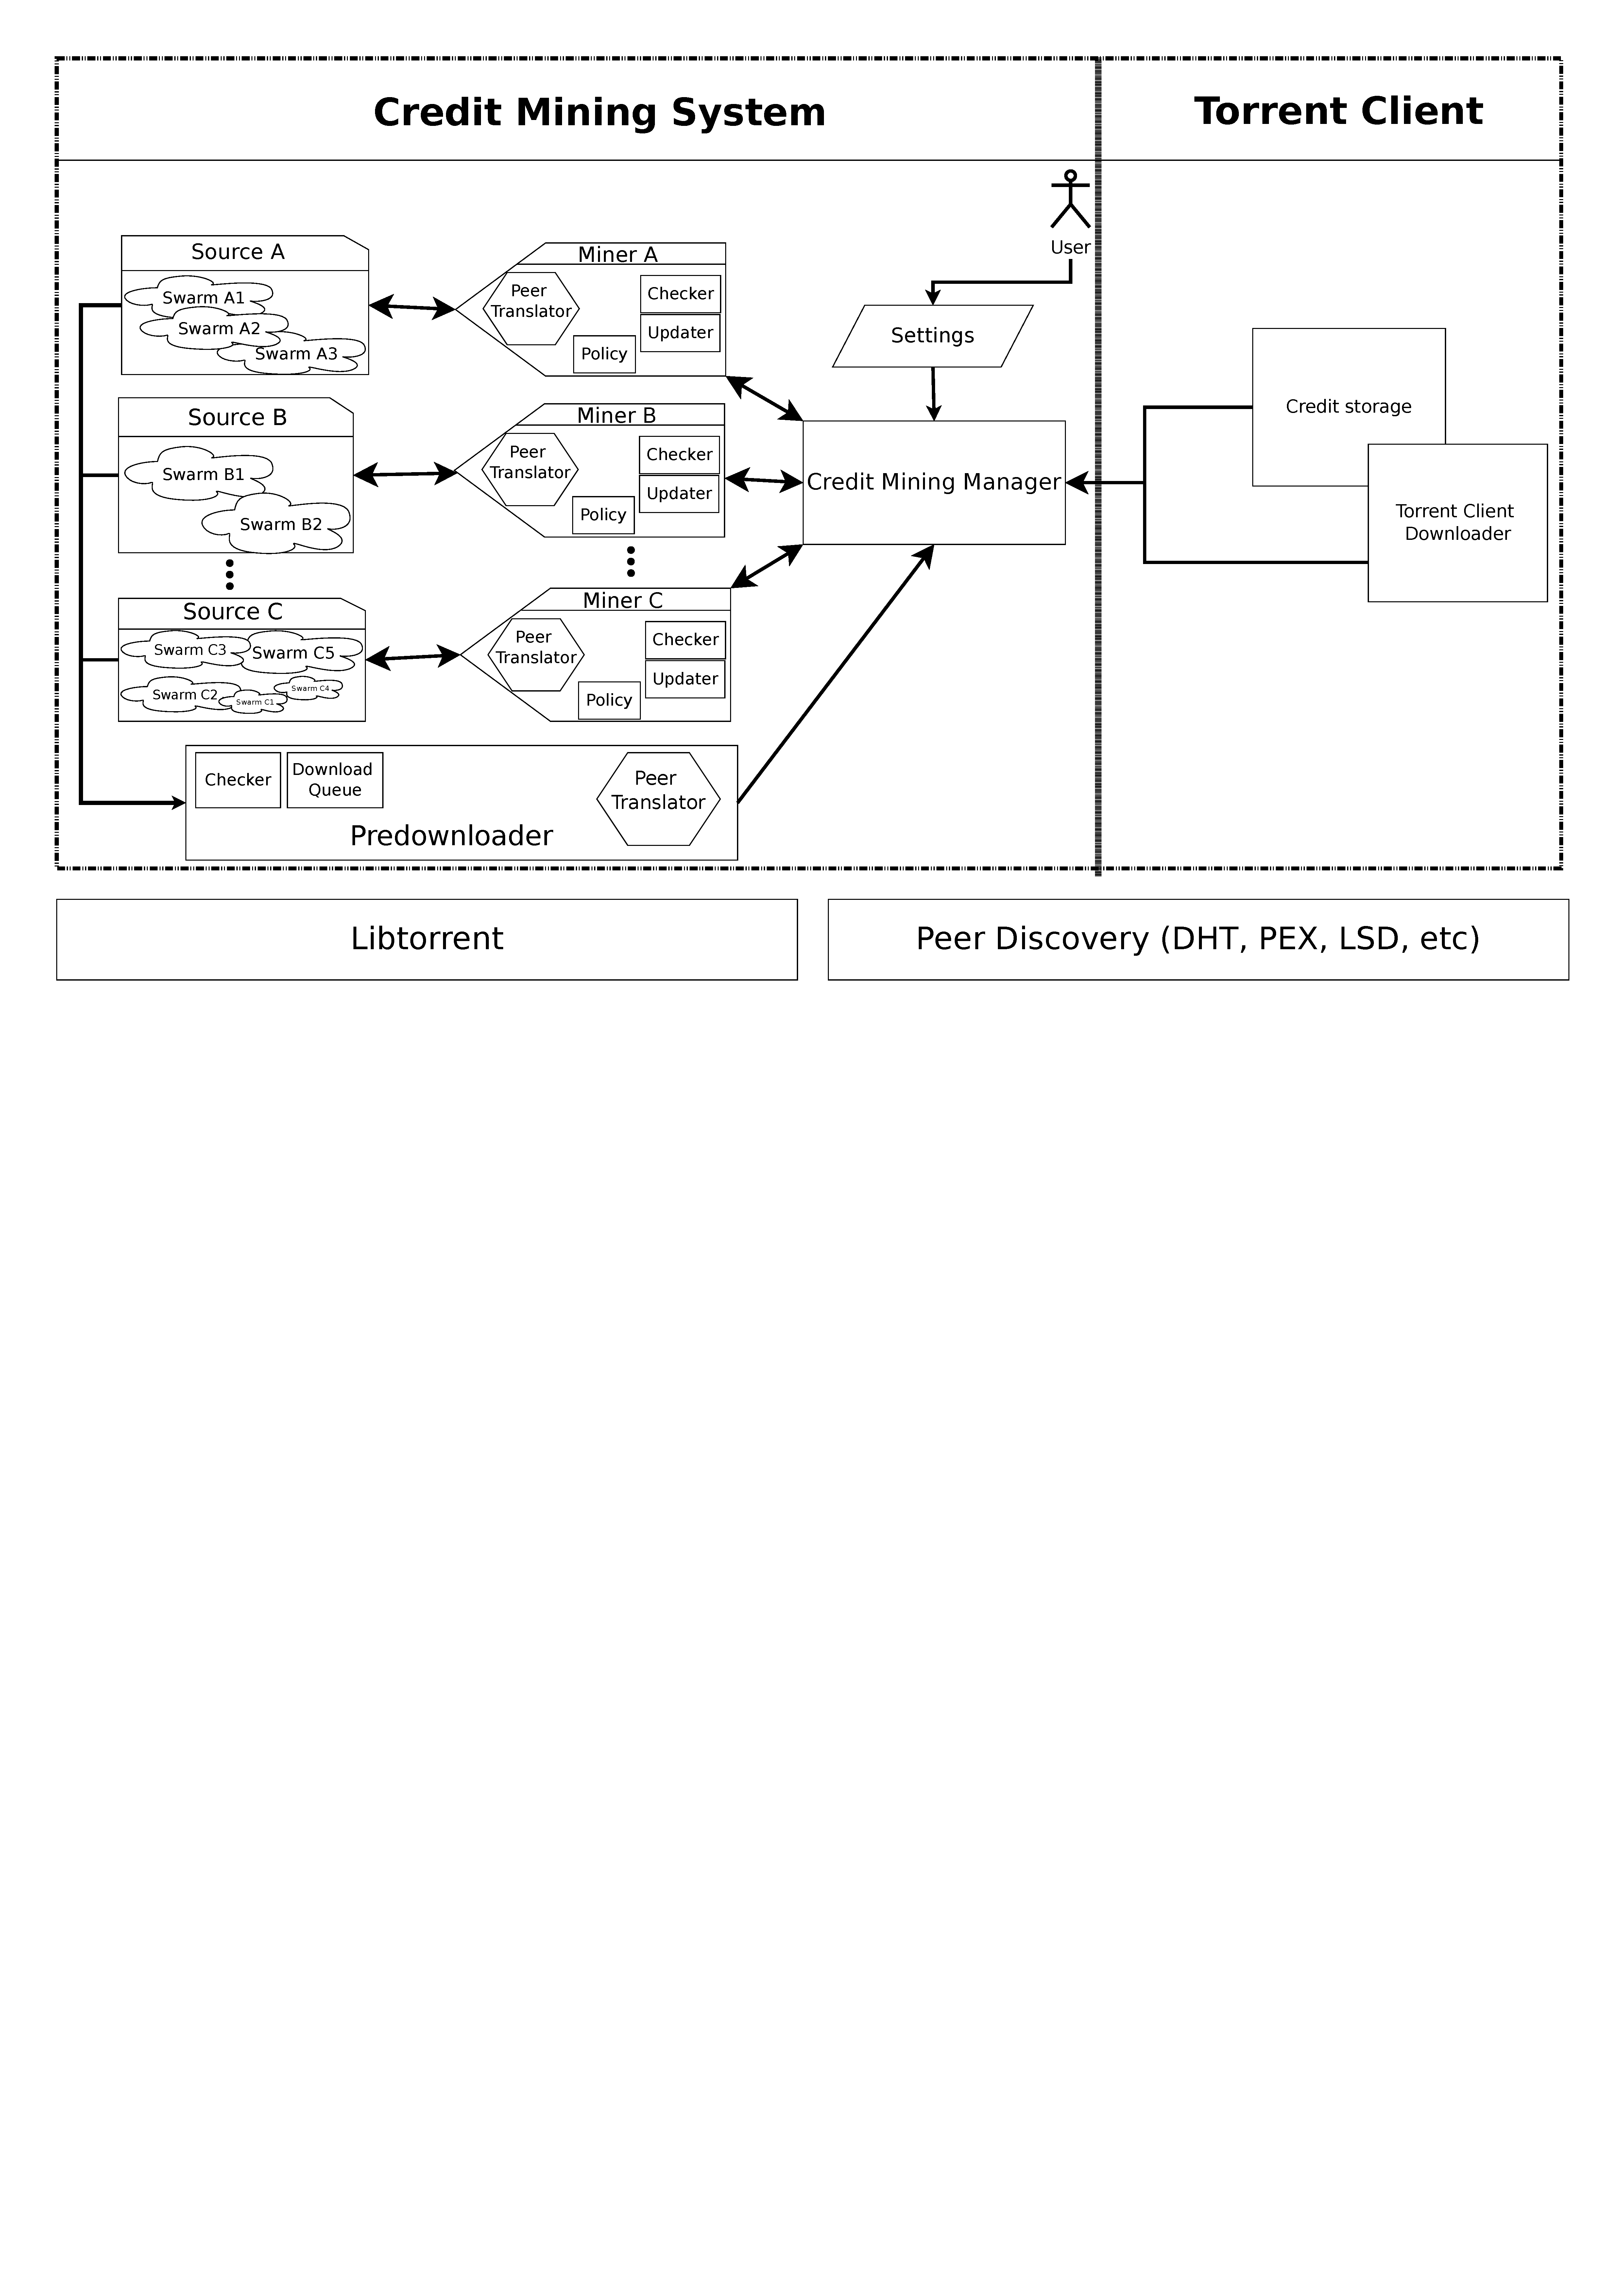
\includegraphics[width=\textwidth]{pics/cm_components.pdf}
	\caption{Credit mining components.}
	\label{fig:cmcomponents}
\end{figure}

% general flow
Before credit mining system is executed, user can change the default settings used in the credit mining system. For example, if user has a lot of memory available, it is desirable to mine many swarms in one time by changing \textit{max\_torrents\_active} parameter. Another example is if user has large storage, decreasing \textit{share\_mode\_target} may result a better return. Some settings can not be changed when mining process run already. Table \ref{tbl:cmsettings} shows the settings used in this system. After user provide the setting and run the \textit{credit manager}, user can start mining by adding sources. A source usually consists of several swarms with different size, availability, and capacity. Each of the source will be assigned with one \textit{miner}. Before the miners start mining, \textit{predownloader} fetches swarm information and then give the results to the manager. Manager will propagate the swarm information to miners and let the miners decide which swarm to mine based on that information. Manager also monitor the main torrent downloader to adjust miners bandwidth allocation. The credit gained from each of the miner will be reported to manager, then it forwards the results to credit storage in torrent client if necessary.

\begin{table}[h]
	\centering
	\caption{Credit mining settings}
	\label{tbl:cmsettings}
	\begin{adjustwidth}{-1.5cm}{}
	\begin{tabular}{|p{1cm}|p{4cm}|p{7cm}|p{2cm}|}
		\hline
		\rowcolor[HTML]{EFEFEF} 
		No. & Name & Description & Changeable at runtime \\ \hline
	1 & \textit{max\_torrents\_active} & The maximum number of simultaneous swarm that will be downloaded & Yes \\ \hline
	2 & \textit{max\_torrents\_per\_source} & The maximum number of stored torrent in a miner that will be considered for mining & Yes \\ \hline
	3 & \textit{source\_interval} & The interval needed to check for updates in the swarm & Yes \\ \hline
	4 & \textit{swarm\_interval} & The interval to re-evaluate swarm and start/stop swarm & Yes \\ \hline
	5 & \textit{share\_mode\_target} & Libtorrent share mode target (See Section \ref{section:sharemode}) & No \\ \hline
	6 & \textit{policy} & The policy used in mining (See Chapter \ref{chapter:prospection}) & No \\ \hline
	7 & \textit{tracker\_interval} & The interval to check for a new peer by peer discovery methods & No \\ \hline
	8 & \textit{timeout\_torrent\_activity} & The maximum time threshold to mark a swarm as 'inactive' & Yes \\ \hline
	9 & \textit{piece\_download} & The number of piece what will be downloaded in \textit{predownload} phase & No \\ \hline
	\end{tabular}
	\end{adjustwidth}
\end{table}



%The rest of this section will discuss key points of credit mining system. Several mining source types are supported with different treatment from miners. Prospecting methodology on top of libtorrent share mode will be elaborated afterwards. The methodology consists of two integral stages. Each of the stage has their own mechanism and requirements. Lastly, we will discuss other components that can support credit mining system of its prospecting, performance, and credit gain. 

\subsection{Mining Sources}
\label{section:msource} 
Currently, credit mining can accommodate three types of sources. There are directory source, RSS source, and channel source. In credit mining system, one source is assigned to one miner. The miner will start working the moment the source is defined and added to the manager. A miner periodically perform checking and other operations on all the swarms in the source.

First type of source which called \textit{directory source}, is very straightforward. It takes a path as an argument and verify it before run the miner. The miner starts by looking at all the file in specified directory that have \texttt{.torrent} file type. Each of the file is examined and validated. Corrupt or invalid file will be discarded and deleted automatically from the disk. In order to keep the performance and prevent disk bottleneck, the miner sort the files alphabetically and put it into queue one by one. Miner periodically monitor both the directory if there is a new file and the queue to assign it to the manager. Miner eventually will pop an item from the queue, build a suitable format for mining, and notify manager to include this swarm.

Next possible mining source is from RSS (Rich Site Summary). RSS is a well known method to fetch new published data from a web. An RSS document contains the list of affected content which usually has summarized text and metadata. An RSS from torrent portal such as etree\footnote{\url{http://bt.etree.org/rss/bt_etree_org.rdf}} and mininova\footnote{\url{http://www.mininova.org/rss.xml}} usually have title, publication date and a link to the swarm. RSS also can easily be generated from private trackers for various purposes. We called a source of RSS document as \textit{RSS feed}. 

In \textit{RSS source}, we assume that the RSS link user provided is available. If by any case the retrieval of the content is failed, the miner will stop immediately, notify the manager to disable this source, and shutting down itself. If the initial content retrieval is successful, update mechanism will be launched periodically to fetch the newest content from the RSS feed. This content then parsed, resulting a list of swarm link and its extra information. Miner then asynchronously download swarm metadata either via \texttt{.torrent} or magnet link. The same metadata will not be downloaded twice. After fetching the data, miner will build a defined format for mining, and then notify manager to include this swarm. 

\textit{Channel source} is the last type of source which tightly related to Tribler environment. As mentioned in section \ref{section:tribler} (Table \ref{tbl:community}), channel is responsible for managing torrents and playlists in Tribler community. A single channel can be discovered in \textit{AllChannel} community. Channel is identified by unique 40-length hexadecimal string. Tribler user can create their own channel, put torrents into the channel, and share to other user. It is also possible for user to add a torrent to another user's channel. When a user subscribe to a channel, they will be notified if new torrent is added into that channel. Moreover, all torrents in subscribed channel will be automatically downloaded into Tribler's database.

Provided the identifier of a channel, miner will continuously try to find and join the channel in \textit{AllChannel}. By joined the channel, miner can get the list of torrents and its properties. After miner joined the channel, the swarm information will be handled and downloaded by Tribler. Miner then monitors the local database whether a new data has been fetched and there is a space for adding possible new torrent to the manager. After knowing swarm information, miner will proceed to download the swarm metadata (\texttt{.torrent} file or magnet link). Afterwards, the mining format will be built and manager will be notified of a ready swarm.

\subsection{User activity awareness}
\label{section:uactivityimpl}
Credit mining is an automatic system to download/upload a swarm. If at the same time, user is downloading a swarm outside the one in credit mining system, the bandwidth will be split. User may experience slower download speed and see this as a problem. We define the \textit{user download activity} as the activity that intentionally initiated by user in order to participate or download content on the particular swarm. Usually, this is the true purpose of having torrent client. 

In response to that issue, we implemented another module in credit mining system to adjust its mining activity to user download activity. Credit mining system periodically observe whether there is a user downloading activity. If there is not any, then it can notify the miners to use all the bandwidth available. In the other case, the system will limit the download and upload rate of mining activity to leftover bandwidth available. At the period of observation, the mining download and upload rate will be set to zero.


\subsection{Resource Optimization}
\label{section:optimization}
In this section, we focus on several optimizations that can be implemented in credit mining system. These optimizations are optional and can be left out. However, as the system itself is not perfect, an improvement to support this system is advantageous. There are three optimization we proposed : duplicate elimination and swarm blacklisting.%, and reusing cache. 

In preliminary work by \citeauthor{2015:creditmining:capota}, credit mining system able to distinguish duplicate content in the P2P communities. It is highly possible that an exact same file have different \textit{infohash} as its identifier. Infohash of a swarm is an SHA1 hash consists of 40 hex character. An \textit{infohash} of a torrent can come from many aspects such as different piece size, categorized as private or public swarm, or even directory name of the files \cite{2015:creditmining:capota}. We used \textit{Levenshtein distance} to measure the different between one swarm and another by considering the files in it. Specifically, its names and length. In the end, we only mine the one who has higher number of seeder. The swarm comparison executed whenever there are new swarm reported by the miners. Eliminating duplicate swarm can lead the peer interaction to be concentrated in one of the swarms. Thus, the performance of participating peer might be improved.

Despite all the features in credit mining system, there is no guarantee that it can constantly gain credit from a particular swarm. The bottleneck in share mode is one of the example. We introduce \textit{swarm blacklisting} to remove and block low performance swarm. Miner periodically watch whether swarms are constantly downloading or uploading data. If no activity detected in a swarm for a long period of time, miner will remove this swarm from its library and block it. That means this swarm can not be chosen by any of the swarm selection policy. It will be added to library again after several rounds. If by any case, the library is empty and there are swarms blacklisted, those will be added to library again.

%In the prior work, it is important to note that after mining for a certain swarm was stopped, miners will delete downloaded files to save the storage. Although it is safe for the system to discard downloaded files, the resource used to redownload piece will be costly. This issue is fixed in current credit mining system. Files from a swarm that has been stopped for mining is archived with its history and stored in \textit{cache}. The history consists of the index of the piece that have been downloaded, peer information, statistics, and many others. When mining restarts, if there are new peers requesting piece the system already have, it can be immediately uploaded without need to redownload or check the piece.